\documentclass[12pt,oneside,letterpaper]{article}

\usepackage[canadien]{babel}
\usepackage[utf8]{inputenc}
\usepackage[T1]{fontenc}
\usepackage{lmodern}
\usepackage{graphicx}
\usepackage[letterpaper]{geometry}
\usepackage{multirow}
\usepackage{caption}
\usepackage{subfig}
\usepackage{hyperref}
\usepackage[all]{hypcap}


\addto\captionsfrench{\def\tablename{Tableau}}
\captionsetup{font=small,labelfont=bf,margin=0.1\textwidth}
\pagestyle{myheadings}
\markboth{GPH-2006/PHY-2002~---~Introduction~à~LabVIEW}{GPH-2006/PHY-2002~---~Introduction~à~LabVIEW}


\begin{document}


\title{\textbf{Complément}\\Introduction à \textit{LabVIEW}}
\author{Jean-Raphaël Carrier \& Claudine Allen}
\date{}
\maketitle


Pour une introduction plus complète au logiciel \textit{LabVIEW}, veuillez vous référer au manuel \textit{Initiation à LabVIEW}. Lorsque vous utiliserez le logiciel, ne vous gênez surtout pas pour consulter les ressources de l'\textit{Aide LabVIEW} (\texttt{Ctrl+?}). De plus, vous pouvez afficher l'\textit{aide contextuelle} (\texttt{Ctrl+H}) ; lorsque vous faites passer le curseur sur un élément du VI, la fenêtre d'aide contextuelle affiche des renseignements sur cet élément.


\section{Introduction}

Un instrument virtuel, ou VI, est un programme fait avec \textit{LabVIEW}. Le terme \textit{instrument virtuel} vient du fait que le fonctionnement et même l'apparence d'un VI s'apparentent grandement à un instrument réel comme un oscilloscope ou un multimètre, par exemple. Non seulement \textit{LabVIEW} peut simuler des appareils, il peut aussi traiter les signaux provenant de vrais instruments et contrôler ces derniers à distance.

Avec le logiciel \textit{LabVIEW}, il y a deux interfaces : l'interface utilisateur (ou face-avant) et le diagramme. La face-avant contient des commandes (boutons, interrupteurs, etc.) et des indicateurs (graphes, voyants lumineux, afficheurs numériques, etc.) ; en bref, la face-avant correspond grossièrement à l'appareil utilisé/simulé. Le diagramme, quant à lui, contient le code qui régit la face-avant. Il est possible de passer rapidement de la face-avant au diagramme et \textit{vice versa} avec \texttt{Ctrl+E}.

\begin{figure}[h]
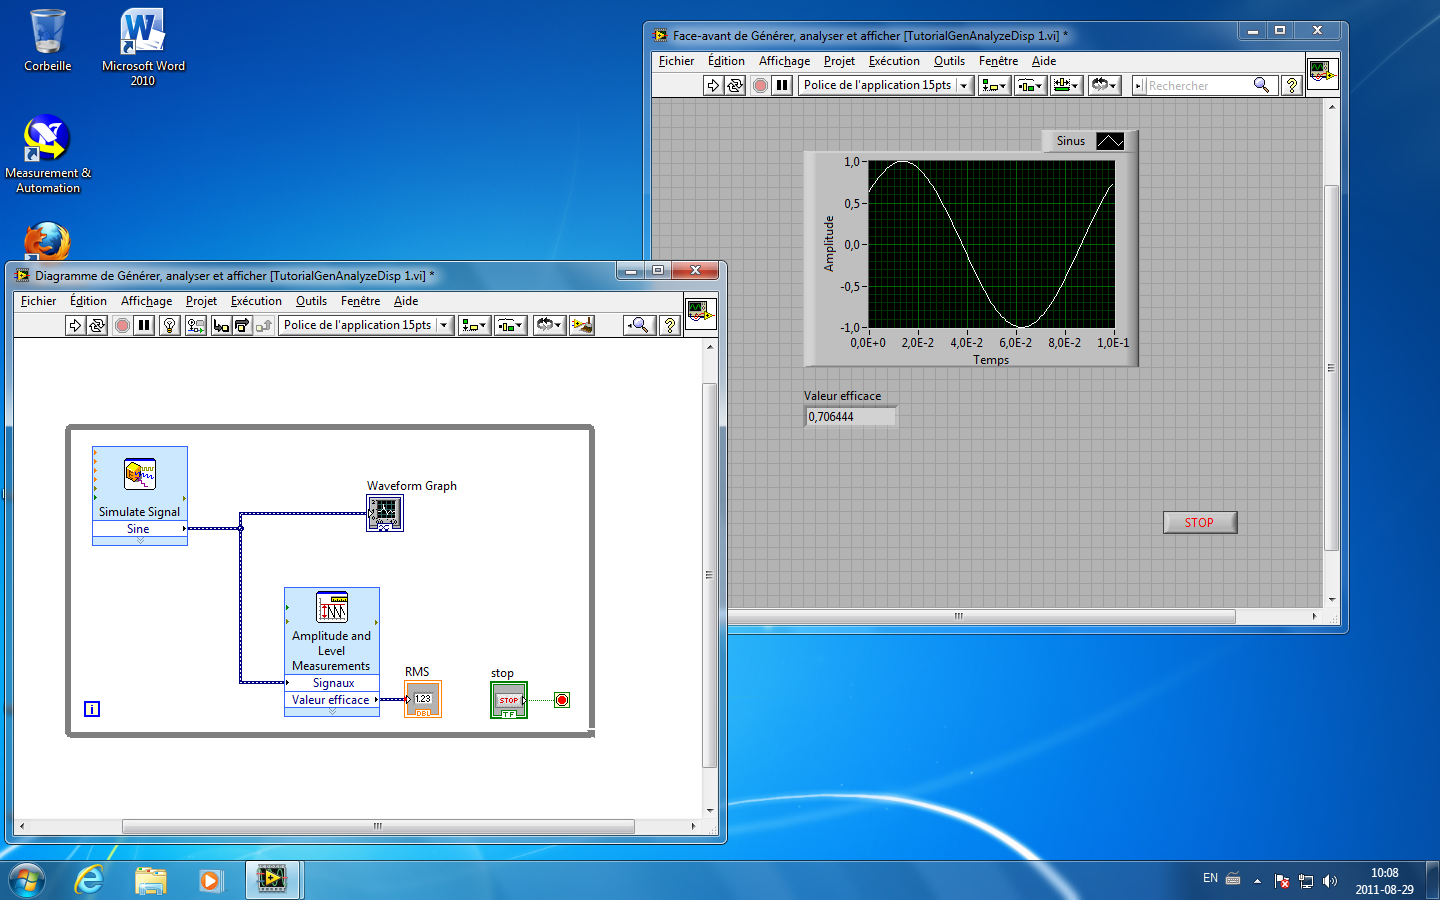
\includegraphics[width=\textwidth]{A classer/LabVIEW-1.png}
\caption{\label{Pauling}Les deux interfaces de LabVIEW : la face-avant (en haut à droite) et le diagramme (en bas à gauche). Ce VI simule un signal sinusoïdal et en calcule la valeur efficace, tout en affichant les résultats sur la face-avant. Le VI s'arrête lorsque l'utilisateur appuie sur le bouton \textsc{stop} (grâce à l'utilisation d'une \textit{boucle While}).}
\end{figure}


\section{Construction d'un VI}

Comme il a été mentionné, la face-avant contient l'interface de l'instrument alors que le diagramme contient le fonctionnement de la face-avant. Ces deux parties sont directement et automatiquement reliées. Par exemple, si vous placez un voyant lumineux sur la face-avant du VI, alors automatiquement vous pourrez voir un icône associé à ce voyant apparaître sur le diagramme. À cet endroit, il sera possible de programmer le code d'entrée du voyant lumineux pour qu'il s'allume pour une condition donnée. Sur le diagramme, les différentes entrées et sorties des composants sont reliées à l'aide de fils, à l'instar d'un circuit électrique.

Il existe toute une liste de fonctions et commandes préfaites dans \textit{LabVIEW}. Les fonctions sont placées sur le diagramme alors que les commandes sont sur la face-avant. Évidemment, celles-ci sont intimement liées. En plus de composants divers, le VI peut en contenir un autre : on parle alors de \textit{sous-VI}. Cette approche modulaire, qui permet «d'emboîter» différents VI, simplifie énormément la construction de VI très complexes.


\section{Structures et boucles}

Les structures et les boucles sont des fonctions qui permettent de régir l'exécution d'un VI ou de certains de ses composants.

Une boucle activera les éléments à l'intérieur de celle-ci lorsqu'elle sera en fonction ; ceux-ci s'arrêteront automatiquement lorsque la boucle sera désactivée. Les boucles permettent d'exécuter plusieurs fois les éléments qu'elle contient : on parle alors d'\textit{itérations}. Une \textit{boucle For} exécute le sous-diagramme qu'elle contient $N$ fois, c'est-à-dire qu'elle fait $N$ itérations. Une \textit{boucle While}, quant à elle, fonctionne jusqu'à ce qu'une condition soit respectée. Ainsi, une boucle While dont la condition d'arrêt est «le nombre d'itérations est égal à 50» est parfaitement équivalente à une boucle For avec $N=50$.

\begin{figure}[h]
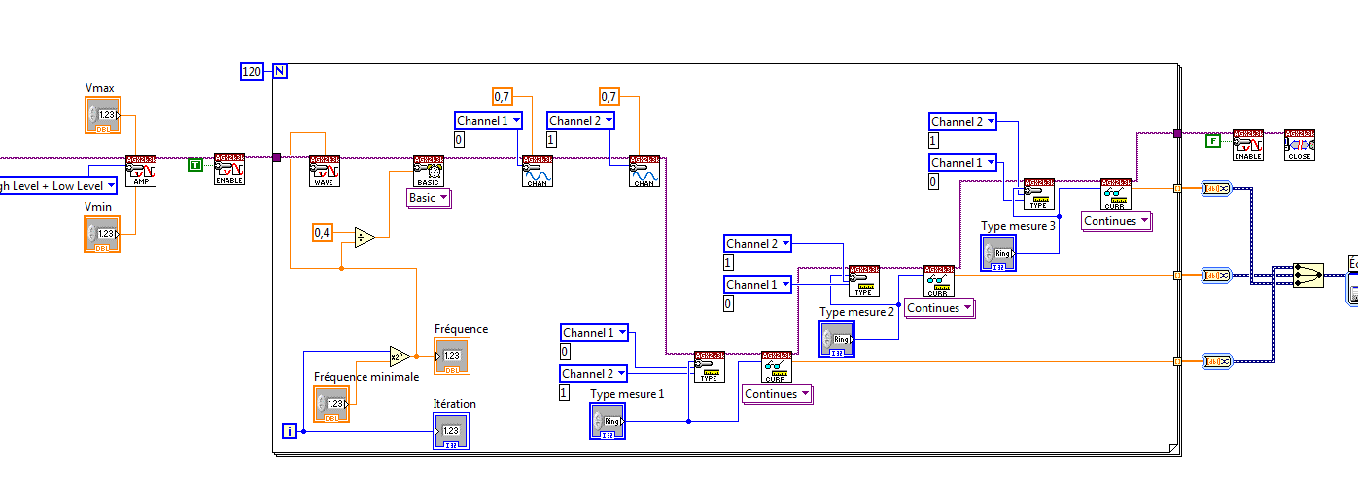
\includegraphics[width=\textwidth]{A classer/LabVIEW-2.png}
\caption{\label{Pauling}Partie d'un diagramme contenant une \textit{boucle For}. Le sous-diagramme à l'intérieur de cette boucle sera exécuté 120 fois.}
\end{figure}

Une structure \textit{séquence} régit l'ordre dans lequel les fonctions doivent être exécutées dans un VI. Cette structure est divisée en cases nommées \textit{étapes}. Les éléments à l'intérieur de la deuxième étape ne seront exécutés que lorsque l'exécution de tous les éléments présents dans la première étape sera terminée. Lorsque la deuxième étape sera terminée, et pas avant, alors les fonctions de la troisième étape s'activeront.

Une structure \textit{condition} peut contenir plusieurs cases aussi appelées \textit{conditions}, dont une seule d'entre elles s'exécute lorsque la structure complète est appelée à s'exécuter. La valeur câblée au terminal de sélection de la structure détermine quel sous-diagramme sera exécuté. Par exemple, une structure condition pourrait être en deux sous-diagrammes, un associé à la valeur \textit{Vrai} et l'autre à la valeur \textit{Faux}. Si la valeur câblée au terminal de la structure est \textit{Vrai}, alors la première case de la structure s'exécute.

\begin{figure}[h]
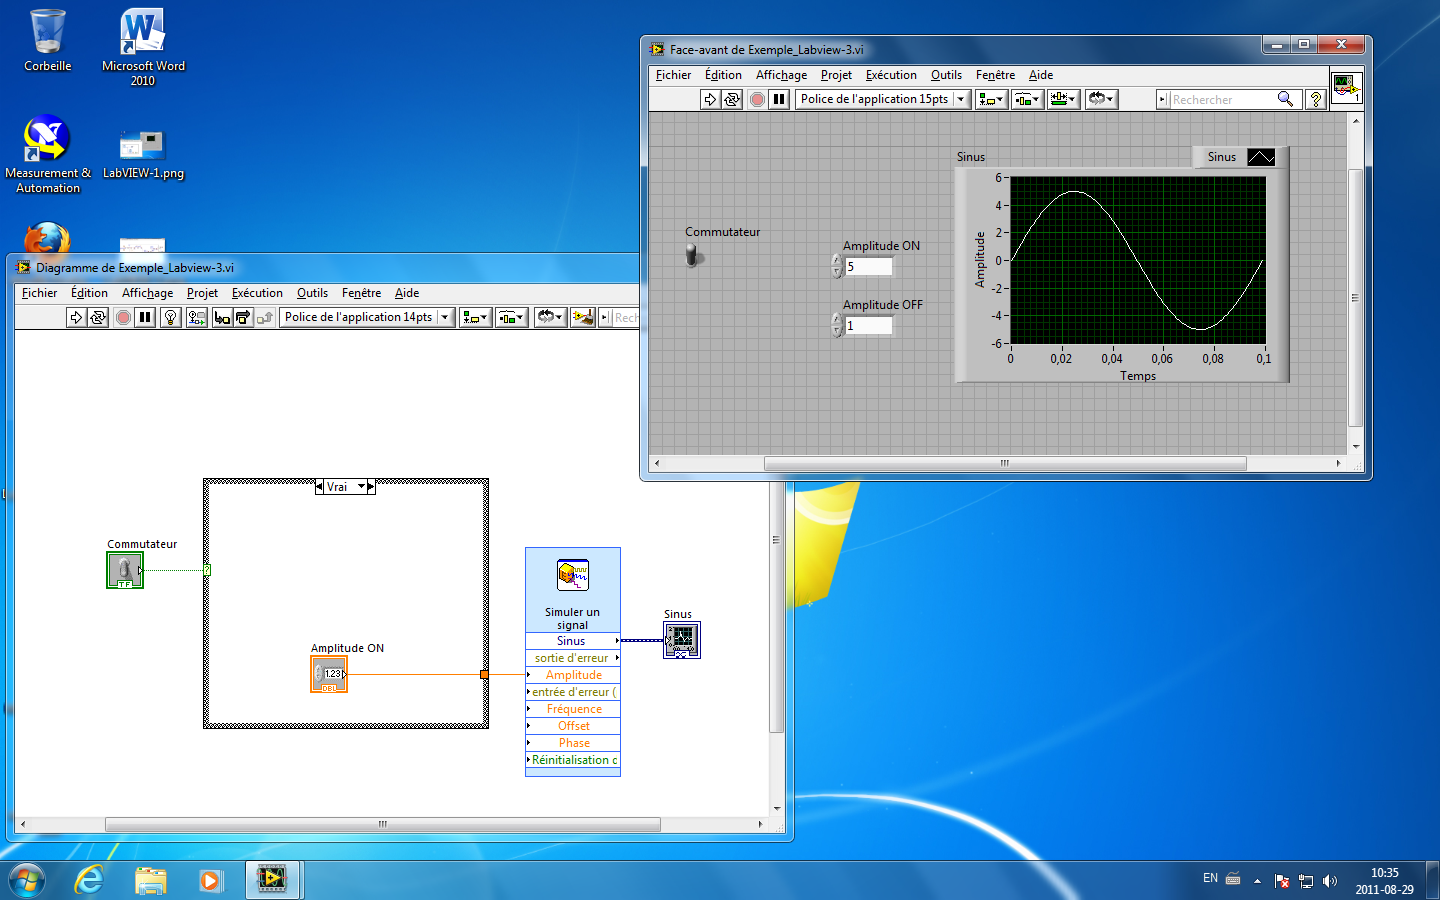
\includegraphics[width=\textwidth]{A classer/LabVIEW-3.png}
\caption{\label{Pauling}VI contenant une structure \textit{condition}. Lorsque le commutateur est à \textsc{on} (valeur \textit{vraie}), l'amplitude du signal sinusoïdal est de 5. Lorsque le commutateur est à \textsc{off} (valeur \textit{fausse}), l'amplitude est de 1.}
\end{figure}

Il existe aussi d'autres sortes de structures et boucles dans \textit{LabVIEW}.


\section{Exécution d'un VI}

Lorsqu'un VI est exécuté (\texttt{Ctrl+R} ou en cliquant sur la flèche en haut à gauche du diagramme ou de la face-avant) en l'absence de structures, tous les éléments sont exécutés une et une seule fois. Un élément n'est exécuté que lorsque toutes ses entrées câblées ont reçu un signal. Les signaux sortant d'un élément ne sont envoyés que lorsque l'exécution de l'élément est complétée. Ceci est vrai aussi pour les boucles et les structures. Ainsi, si deux signaux entrent dans une boucle For et que trois en sortent, alors l'exécution de la boucle ne commence que lorsqu'elle aura reçu un signal provenant de chacune de ses deux entrées, donc à la fin de leur exécution. Lorsque la boucle a terminé d'exécuter toutes ses itérations, et seulement alors, elle envoie ses trois signaux de sortie.

Ainsi, avec \textit{LabVIEW}, la façon dont les éléments sont placés et câblés détermine l'ordre dans lequel ils sont exécutés. Ces éléments peuvent être en série ou en parallèle. Dans le premier cas ils s'exécutent l'un après l'autre, alors que dans le deuxième cas, toutes les exécutions se font simultanément.


\section{Types de signaux}

Il existe différents types de signaux dans \textit{LabVIEW}, d'où un élément ne peut pas nécessairement être relié avec n'importe quel autre : les types de signaux doivent concorder. Par exemple, si une fonction envoie un signal qui peut seulement être \textit{Vrai} ou \textit{Faux}, il ne pourra pas être géré par une fonction qui prend une valeur numérique et la multiplie par un autre nombre.

Les signaux simples peuvent être un nombre, une ligne de texte, une valeur booléenne (\textit{Vrai} ou \textit{Faux} --- 1 ou 0), etc. Un signal peut aussi être un \textit{array} ou un \textit{cluster}. Dans les deux cas, le signal est composé de plusieurs valeurs. Un \textit{array} est une matrice faite de signaux de même type ; des opérations mathématiques peuvent donc être faites directement avec ce type de signal. Un \textit{cluster} est un ramassis de valeurs pouvant être de différents types: poèmes de Nelligan, les 46 premiers chiffres de $\pi$, le secret de la Caramilk, la combinaison du coffre-fort de votre grand-mère, un \textit{array}, n'importe quoi peut faire partie d'un \textit{cluster}! Il s'agit ainsi d'une sorte de banque d'information pouvant être enregistrée dans un fichier, mais ne pouvant pas subir d'opérations directement dans un VI.

\textit{LabVIEW} possède un code de grosseurs et de couleurs, résumé dans le tableau~\ref{tab-types-signaux}, qui permet de reconnaître, au premier coup d'oeil, le type de signal qui est contenu dans un fil.

\begin{table}[h]
\begin{center}
\begin{tabular}{|c|c|}
\hline
\textbf{Caractéristique du lien} & \textbf{Signification} \\
\hline
fil mince & signal simple (une seule valeur) \\
\hline
fil épais & signal composé (\textit{array} ou \textit{cluster}) \\
\hline
fil vert & valeur booléenne (\textit{Vrai}/\textit{Faux} --- 1/0) \\
\hline
fil bleu & valeur numérique entière \\
\hline
fil orange & valeur numérique réelle \\
\hline
fil jaune & signal d'erreur \\
\hline
fil rose & ligne de texte \\
\hline
fil mauve & adresse d'un appareil \\
\hline
\end{tabular}
\end{center}
\caption{\label{tab-types-signaux}Code de grosseurs et de couleurs des différents types de signaux dans \textit{LabVIEW}.}
\end{table}


\section{Acquisition et traitement des données}

\textit{LabVIEW} s'avère très utile lorsqu'une acquisition de données est nécessaire dans une expérimentation. Supposons qu'on veuille mesurer le courant qui circule dans une résistance électrique en fonction de la température, tout en appliquant une tension constante. Si la source de tension, le système qui fait varier la température, le capteur de température ainsi que l'ampèremètre sont compatibles avec \textit{LabVIEW}, alors toute cette manipulation pourra être programmée avec le logiciel : vous n'aurez même pas à vous lever de votre chaise! Avec une fonction, vous pourrez fixer la tension aux bornes de la résistance et avec une autre, vous pourrez mettre en marche le système qui fait varier la température (un système Peltier, par exemple). Par la suite, vous pourrez lire la température avec des acquisitions successives du capteur et commander l'ampèremètre afin qu'il lise la valeur du courant à chaque fois que la température augmente de 1~°C. Enfin, le programme pourra arrêter cette acquisition automatiquement lorsque la température atteint une certaine valeur, choisie à l'avance.

\textit{LabVIEW} peut aussi débuter le traitement des données en effectuant des calculs, en construisant des graphiques, des tableaux, à partir des données brutes acquises. Les résultats de ces traitements peuvent être affichés sur la face-avant. Le VI peut aussi enregistrer toutes les données, brutes et/ou traitées, dans un fichier qui pourra par la suite être lu avec des logiciels comme \textit{Excel} ou \textit{MATLAB}.


\end{document}


Écrit par Jean-Raphaël Carrier
Dernière modification : 9 janvier 2014

Reste à faire:

- (à voir) Rajouter un tableau de conversion anglais-français de LabVIEW

